\subsection{提案手法 概要}
提案手法の概要図を\figref{fig:proposed_method}に示す.
本手法では, 入力スパイク列$\bm{o}(t)$の未学習の速度に対して, その推論精度が低下しにくいSNNを実現することを目指す.
一般的に, ニューラルネットワークは入力の加減速に対して, その内部状態は単純な加減速とはならない.
そのため, ニューラルネットワークの最終的な出力は, 入力の速度変化に依存して変化する.
そこで本手法では, 入力の速度変化に応じて, SNNの内部状態の変化量を動的に調整する機構を導入する.
内部状態の変化量の調整は, 時定数$\tau$を含むSNNのパラメータ (\figref{fig:proposed_method}における$\tau', r'$) を推定器で推定し, その推定値を適用することで行う.
この機構によって, 入力速度変化による内部状態の変化を抑制し, 頑健な推論を行うSNNを構築する.

\begin{figure}[htb]
    \centering
    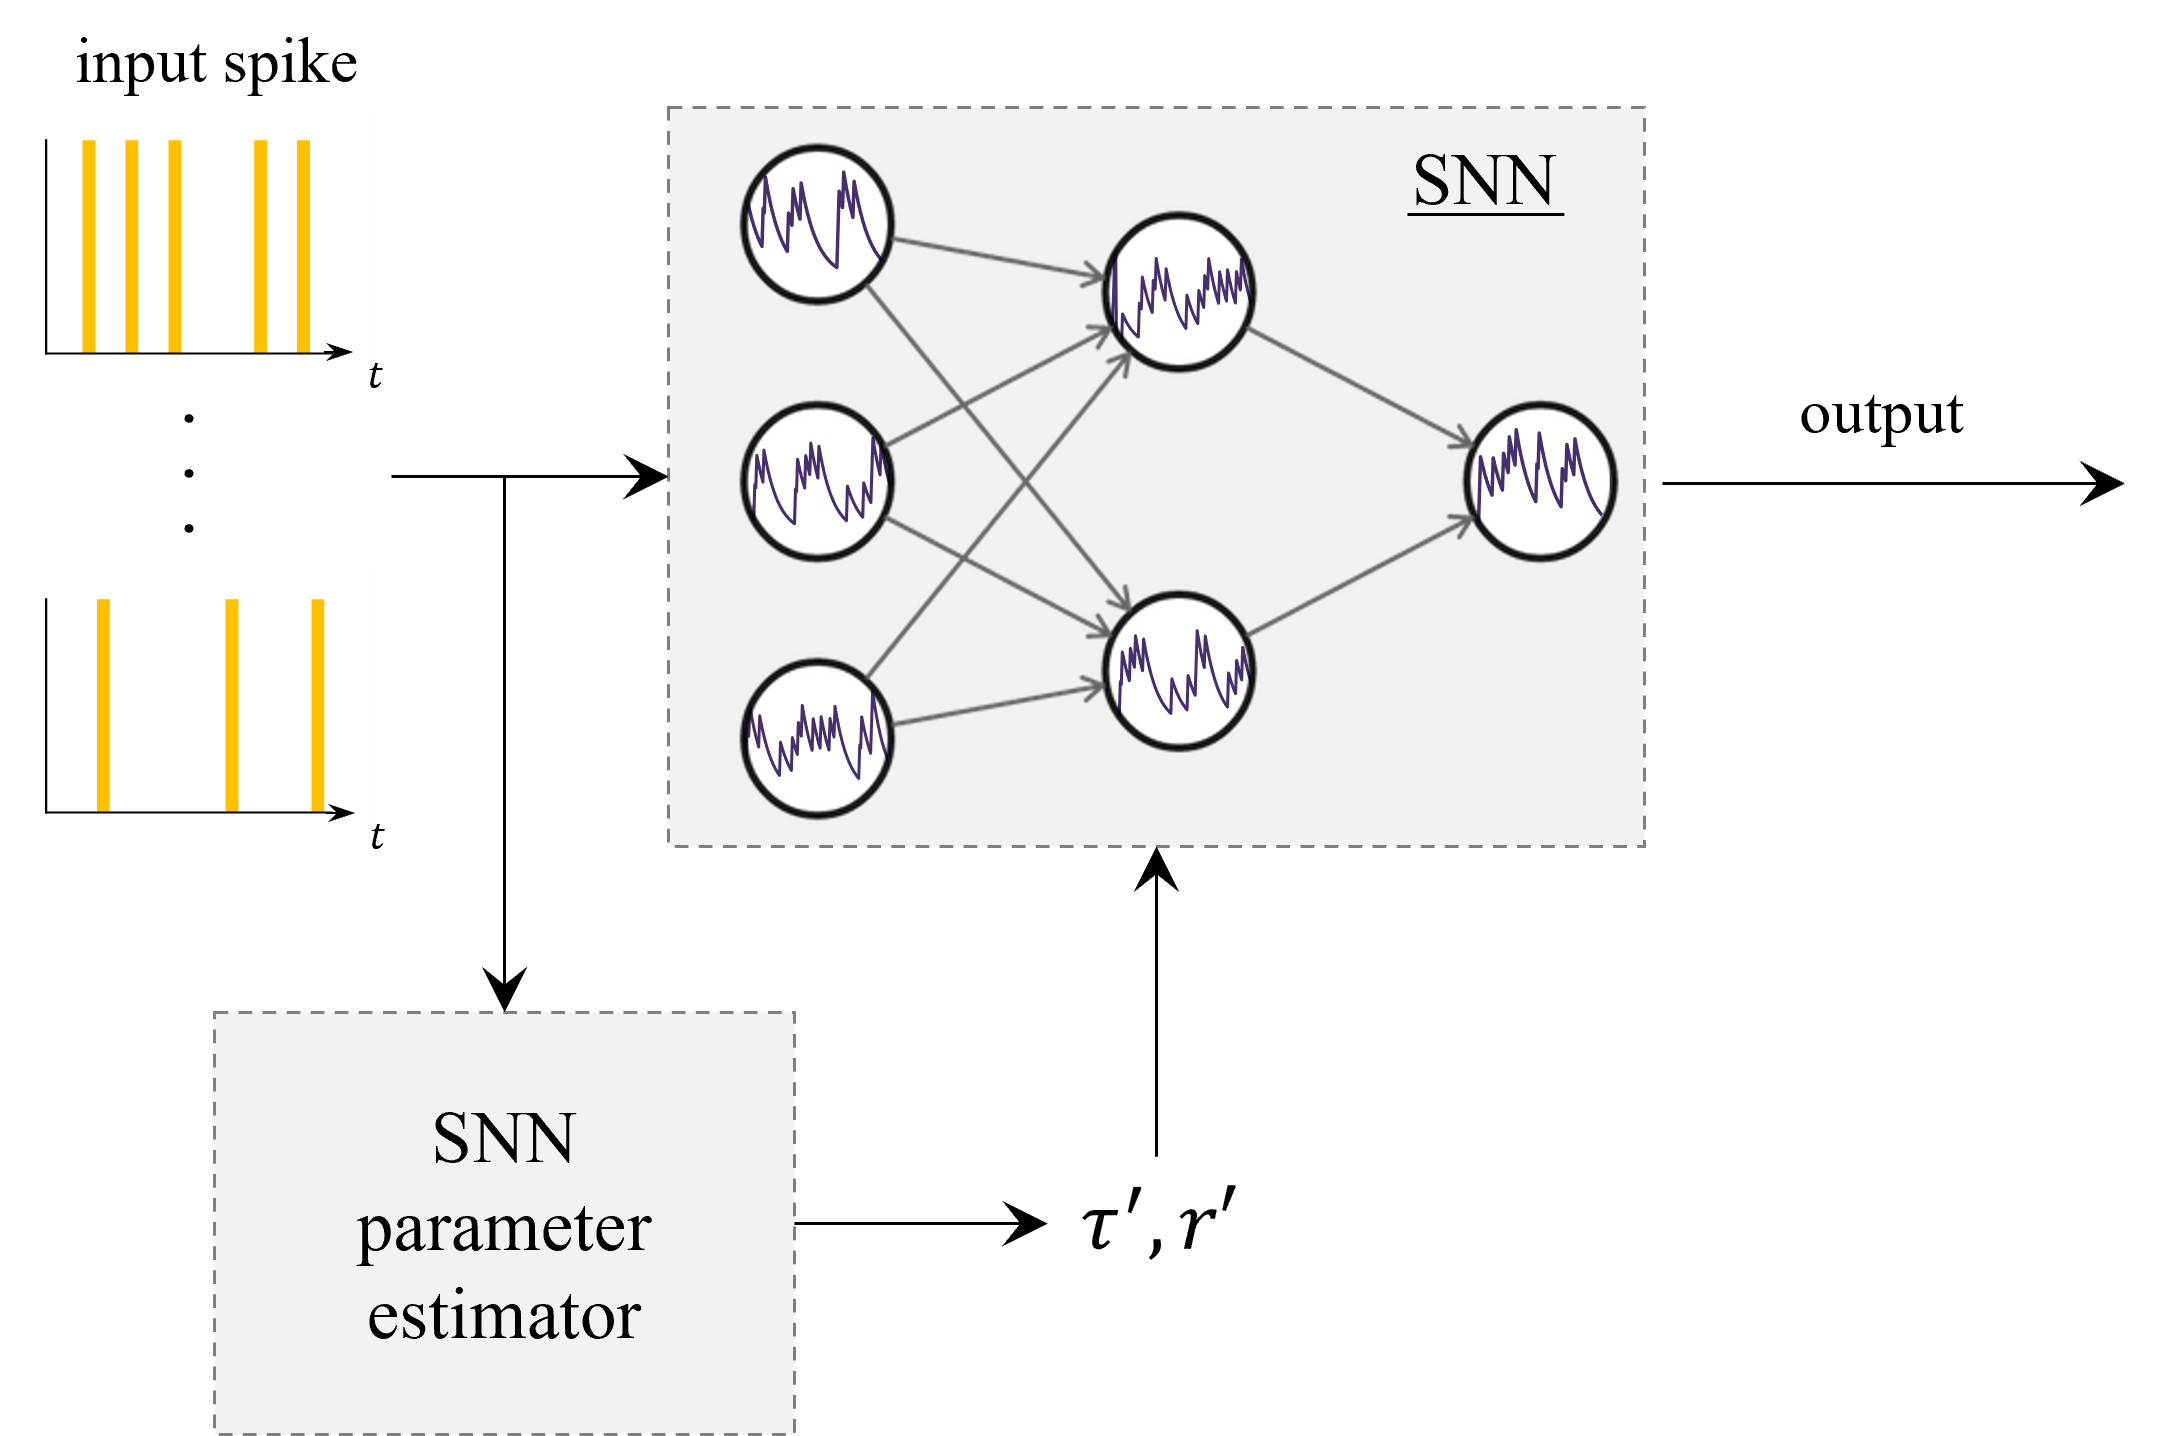
\includegraphics[width=0.9\textwidth]{Static/chap2_sec2_methodstr.png}
    \caption[提案手法の概要図]{
        提案手法の概要図.
        $\tau', r'$はそれぞれ時定数$\tau$と膜抵抗$r$の推定値を表す.
    }
    \label{fig:proposed_method}
\end{figure}

提案手法の導出は以下の3ステップで行う.
\begin{enumerate}
    \item 入力スパイク列の速度変化に対する理想的なSNNの内部状態の定式化
    \item 入力スパイク列の速度変化に対する実際のSNNの内部状態の定式化
    \item 実際の内部状態を理想的な内部状態に近似するための条件の導出
\end{enumerate}
ここで, 理想的なSNNの内部状態とは, 入力スパイク速度が$a$倍になった場合に, 内部状態の変化速度も$a$倍になることを意味する.
実際の内部状態を理想的な内部状態に近似できる条件を導出 (\figref{fig:proposed_method_intro}) し, その条件を満たすようにSNNの時定数および膜抵抗の値を推定することで, 入力速度変化による内部状態の変化を抑制する.
\begin{figure}[htb]
    \centering
    \includesvg[width=0.9\textwidth, inkscapelatex=false]{Static/chap2_sec2_methodintro}
    \caption[提案手法の導出の概要図]{
        提案手法の導出の概要図.
        $v(at), v(t)$はそれぞれ理想的なSNNの内部状態と実際のSNNの内部状態を表す.
    }
    \label{fig:proposed_method_intro}
\end{figure}


